\documentclass[11pt,a4paper]{article}

\usepackage[utf8]{inputenc}
\usepackage{fullpage}
\usepackage{authblk}
\usepackage{graphicx}
\usepackage{caption}
\usepackage{subcaption}
\usepackage{amsmath}
\usepackage{amssymb}
\usepackage{bbm}
\usepackage{euscript}
\usepackage{graphicx}
\usepackage{subcaption}
\usepackage{lmodern}
\usepackage{textcomp}
\usepackage{titlesec}
\usepackage{float}
\usepackage{amsfonts}
\usepackage{bm}
\usepackage{stmaryrd}
\usepackage{bbm}

% red
% R: 202 G: 53 B: 66 
% \definecolor{myred}{rgb}{0.789,0.207,0.2578}

% blue
% R: 39 G: 100 B: 123
% \definecolor{myhyperblue}{rgb}{0.152,0.39,0.48}

% green
% R: 132 G: 159 B: 173
% \definecolor{mygreen}{rgb}{0.5156,0.62,0.6757}

\usepackage{color}
\definecolor{myorange}{rgb}{0.9568,0.4941,0.1961}
\definecolor{myred}{rgb}{0.9098,0.1294,0.2078}
\definecolor{myblue}{rgb}{0.0352,0.4981,0.6509}
\definecolor{mygreen}{rgb}{0.2235,0.6353,0.2588}
\definecolor{lightgray}{rgb}{0.8,0.8,0.8}
\definecolor{myhyperblue}{rgb}{0.1607,0.3922,0.9}
\definecolor{mygrey}{rgb}{0.3,0.3,0.3}

\newcommand{\unknown}[1]{\bm{{\color{myred}{#1}}}}
\newcommand{\param}[1]{\bm{{\color{myhyperblue}{#1}}}}
\newcommand{\data}[1]{\bm{{\color{mygreen}{#1}}}}
\newcommand{\keyword}[1]{[\texttt{\textbf{#1}}]\!\,}

\title{Functional scope \texttt{wave1D v1}: piezoelectric models}

\author[1]{Florian Le Bourdais, Alexandre Imperiale}

\begin{document}

% \bibliographystyle{apalike}

\maketitle

\section{Continuous models}
\subsection{Strong formulations}
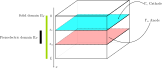
\includegraphics[scale=1]{figures/1dstack.png} 

Domains: 

Let $\Omega_S$ be the solid domain.
Let $\Omega_P$ be the piezoelectric domain, under the assumption that  $\Omega_P \subset  \Omega_S$.

\begin{equation*}
\quad \quad
\keyword{Piezo}~
\left\lbrace
\begin{aligned}
& \param{\rho}\partial^2_{tt} \unknown{u} - \partial_x\big( \param{E} \partial_x \unknown{u} \big) = \partial_x\big( \param{d} \partial_x \unknown{\varphi} \big) + \data{f},\quad \text{in }\Omega_S,\\
& \partial_x\big( \param{\varepsilon} \partial_x \unknown{\varphi} \big) =  \partial_x\big( \param{d} \partial_x \unknown{u} \big),\quad \text{in }\Omega_P,\\
\end{aligned}
\right.
\end{equation*}<

In the above, $\param{\rho}$ is the mass density, $\param{E}$ is the Young modulus, $\param{d}$ is the piezoelectric coupling factor and $\param{\varepsilon}$ is the electric permittivity.

Boundary conditions:

Initial conditions:


\end{document}
